\chapter{Análisis de requisitos}
\label{cap:analisis}

Este capítulo describe el análisis funcional del sistema desarrollado en
este proyecto, en el capítulo se describen: los actores que interactúan con él, los requisitos de
información, los requisitos funcionales y no
funcionales que debe satisfacer, las reglas de negocio, y los casos de uso que formalizan cómo se usa. 
Finalmente el capítulo
se cierra con una matriz de trazabilidad que relaciona cada requisito con
los objetivos específicos definidos en la
sección~\ref{sec:intro-objetivos} del capítulo~\ref{cap:introduccion},
de modo que pueda comprobarse que ningún objetivo queda sin cubrir y que
ningún requisito queda fuera de los fines del proyecto.

\section{Contexto funcional del sistema}
\label{sec:analisis-contexto}

El sistema desarrollado en este proyecto aborda la comparación de
algoritmos de seguimiento multiobjeto sobre vídeo de fútbol y la extracción
de metadatos deportivos a partir de las trayectorias resultantes. Se
organiza en dos bloques con una naturaleza muy distinta, representados en
la Figura~\ref{fig:analisis-contexto}: un \textbf{pipeline offline} en
Python, que concentra todo el cómputo pesado, y una
\textbf{aplicación web} de visualización (sección~\ref{sec:implementacion-web}),
que consume los resultados ya calculados por el pipeline. El planteamiento se detalla en el
capítulo~\ref{cap:diseno}.

\begin{figure}[htp]
\centering
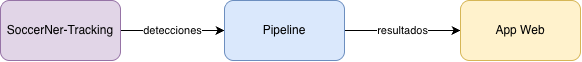
\includegraphics[width=0.7\textwidth]{figures/contexto_funcional.drawio.png}
\caption{Contexto funcional del sistema: el dataset público como entrada, el
pipeline offline como bloque de cómputo, y la aplicación web como capa de
visualización sobre los resultados.}
\label{fig:analisis-contexto}
\end{figure}

\subsection{Justificación y decisión de la tarea elegida}
\label{sec:analisis-decision}

Antes de comprometerse con el seguimiento multiobjeto como tarea de este
proyecto, se exploraron brevemente otras tareas del ecosistema SoccerNet, como parte de la primera fase del
proyecto descrita en la sección~\ref{sec:gestion-fases}. Concretamente, se
valoraron tres alternativas:

\begin{itemize}
  \item \textbf{Reconocimiento de dorsales} (\emph{jersey number
        recognition}): predecir el número de un jugador a partir de una
        imagen recortada. Se consideró una opción técnicamente válida y de
        alta viabilidad que era adecuada para el contexto del proyecto, ya
        que trataba de trabajar sobre imágenes estáticas, no sobre
        secuencias, pero con menor profundidad técnica para una
        comparativa de algoritmos, el enfoque que finalmente se decidió dar
        a este proyecto.
  \item \textbf{Segmentación de cámara} (\emph{camera segmentation}):
        clasificar en cada instante del vídeo el tipo de plano de cámara
        (plano general, primer plano, repetición). Se descartó sin llegar a
        explorarse ni implementarse: se valoró como menos interesante
        técnicamente y de menor impacto visual en una demostración que las
        otras dos alternativas.
  \item \textbf{Seguimiento multiobjeto} (MOT, sección~\ref{sec:fundamentos-mot}):
        la tarea finalmente elegida.
\end{itemize}

La decisión final se apoyó en varios factores concretos, verificados
mediante pruebas exploratorias reales antes de comprometerse con la tarea:
el dataset SoccerNet-Tracking incluye detecciones ya calculadas, lo
que elimina la barrera de tener que entrenar o adaptar un detector de
objetos propio; en apenas unas horas de exploración inicial fue posible
pasar de cero a visualizaciones funcionales sobre el \emph{ground truth}; el
tutor confirmó que era válido plantear el trabajo como una comparativa
rigurosa de varios algoritmos de \emph{tracking-by-detection}
(sección~\ref{sec:fundamentos-algoritmos}), en lugar de limitarse a
implementar uno solo; y la posibilidad de una demostración web con mapa de
calor de trayectorias se valoró como la más atractiva visualmente de las
tres alternativas exploradas.

Como consecuencia directa de esta decisión, y como se ha detallado en la
sección~\ref{sec:fundamentos-algoritmos}, se seleccionó la librería
\texttt{boxmot}, la cual agrupa varias implementaciones de algoritmos de
tracking bajo una interfaz común, de modo que cambiar de algoritmo se
reduce a cambiar una línea de código, ideal para una comparativa, fijando
específicamente su versión \texttt{10.0.43}, ya que versiones posteriores
de la librería (a partir de la v18) dejaron de mostrar las clases de cada
algoritmo por separado, unificándolas bajo una única interfaz, lo cual no se
quería en este proyecto, ya que dificultaba precisamente la comparación que el proyecto
necesitaba. Para la evaluación se adoptó \texttt{TrackEval}, por ser la herramienta de
referencia oficial del propio benchmark de SoccerNet y que funciona muy bien con el formato MOT estándar que produce \texttt{boxmot}.

\section{Actores y usuarios del sistema}
\label{sec:analisis-actores}

La aplicación web, una vez
desarrollada, consumirá artefactos estáticos sin sesión de usuario. Por
ese motivo, los actores no son usuarios con inicio de sesión, sino roles o
perspectivas de uso frente al sistema. En el desarrollo, es solo el autor del proyecto quien
asume los roles internos, pero
se describen por separado porque responden a objetivos distintos frente al
sistema, del mismo modo que se distinguieron los roles de gestión en la
sección~\ref{sec:gestion-roles}.

Se identifican dos actores primarios y un actor secundario, representados
en la Figura~\ref{fig:analisis-actores} y descritos en la
Tabla~\ref{tab:analisis-actores}: el \textbf{operador del pipeline}, que
ejecuta las distintas fases del procesamiento offline, el \textbf{usuario
analista} que consulta la aplicación web para explorar e interpretar los
resultados y SoccerNet, como sistema externo del
que el pipeline obtiene los datos de entrada.

\begin{figure}[htp]
\centering
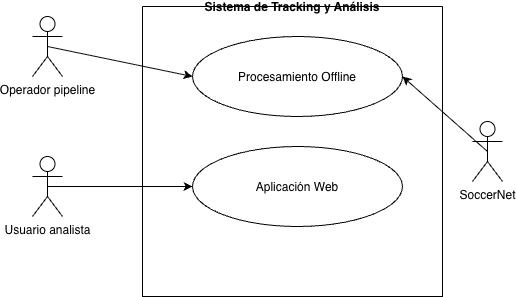
\includegraphics[width=0.7\textwidth]{figures/diagrama_actores.drawio.png}
\caption{Actores del sistema: operador del pipeline y usuario analista
(izquierda), interactuando respectivamente con el procesamiento offline y
la aplicación web, y SoccerNet como sistema externo (derecha).}
\label{fig:analisis-actores}
\end{figure}

\begin{table}[htp]
\centering
\caption{Actores y usuarios del sistema.}
\label{tab:analisis-actores}
\renewcommand{\arraystretch}{1.3}
\begin{tabular}{|p{2.7cm}|p{1.7cm}|p{7.9cm}|}
\hline
\rowcolor{gray!25}
\textbf{Actor} & \textbf{Tipo} & \textbf{Descripción} \\
\hline
Operador del pipeline & Primario &
  Ejecuta las fases del procesamiento offline: descarga del dataset,
  tracking, evaluación, estudio de hiperparámetros y extracción de
  metadatos. \\
\hline
Usuario analista & Primario &
  Consulta la aplicación web para explorar los vídeos
  anotados, las métricas comparativas y los metadatos deportivos
  generados. \\
\hline
SoccerNet & Secundario &
  Sistema externo del que se obtienen las secuencias de vídeo, las
  detecciones precomputadas y el \emph{ground truth}
  (sección~\ref{subsec:fundamentos-soccernet-tracking}). \\
\hline
\end{tabular}
\end{table}

\section{Requisitos de información}
\label{sec:analisis-irq}

Los requisitos de información indican qué datos debe recopilar, generar y
conservar el sistema para ejecutar el pipeline. Se recogen en las Tablas~\ref{tab:irq-001}
a~\ref{tab:irq-009}.

\begin{table}[htp]
\centering
\caption{IRQ-001: Detecciones precomputadas de SoccerNet-Tracking.}
\label{tab:irq-001}
\renewcommand{\arraystretch}{1.2}
\begin{tabular}{|p{3.1cm}|p{9.2cm}|}
\hline
\rowcolor{gray!25}
\multicolumn{2}{|l|}{\textbf{IRQ-001 -- Detecciones precomputadas de SoccerNet-Tracking}} \\
\hline
Versión & v1.0 \\
\hline
Rol & Operador del pipeline \\
\hline
Datos específicos & \texttt{frame\_id}, \texttt{x}, \texttt{y}, \texttt{w},
  \texttt{h}, \texttt{confianza} (fichero \texttt{det.txt} por secuencia) \\
\hline
Descripción & El sistema debe leer, para cada secuencia, las detecciones ya
  calculadas de jugadores, árbitros y balón, como entrada de los
  algoritmos de tracking (sección~\ref{sec:fundamentos-mot}). \\
\hline
\end{tabular}
\end{table}

\begin{table}[htp]
\centering
\caption{IRQ-002: \emph{Ground truth} de tracking.}
\label{tab:irq-002}
\renewcommand{\arraystretch}{1.2}
\begin{tabular}{|p{3.1cm}|p{9.2cm}|}
\hline
\rowcolor{gray!25}
\multicolumn{2}{|l|}{\textbf{IRQ-002 -- \emph{Ground truth} de tracking}} \\
\hline
Versión & v1.0 \\
\hline
Rol & Operador del pipeline \\
\hline
Datos específicos & \texttt{frame\_id}, \texttt{obj\_id}, \texttt{x},
  \texttt{y}, \texttt{w}, \texttt{h} (fichero \texttt{gt.txt}, solo en
  train y test) \\
\hline
Descripción & El sistema debe leer la posición e identidad real de cada
  objeto por frame, como referencia para calcular las métricas de
  evaluación (sección~\ref{sec:fundamentos-metricas}). \\
\hline
\end{tabular}
\end{table}

\begin{table}[htp]
\centering
\caption{IRQ-003: Metadatos de secuencia y de partido.}
\label{tab:irq-003}
\renewcommand{\arraystretch}{1.2}
\begin{tabular}{|p{3.1cm}|p{9.2cm}|}
\hline
\rowcolor{gray!25}
\multicolumn{2}{|l|}{\textbf{IRQ-003 -- Metadatos de secuencia y de partido}} \\
\hline
Versión & v1.0 \\
\hline
Rol & Operador del pipeline \\
\hline
Datos específicos & Resolución de imagen y \emph{frame rate}
  (\texttt{seqinfo.ini}); \\
\hline
Descripción & El sistema debe conservar esta información de contexto de
  cada secuencia, necesaria para interpretar correctamente sus detecciones
  y para la configuración de \texttt{TrackEval}. \\
\hline
\end{tabular}
\end{table}

\begin{table}[htp]
\centering
\caption{IRQ-004: Resultados de tracking por algoritmo.}
\label{tab:irq-004}
\renewcommand{\arraystretch}{1.2}
\begin{tabular}{|p{3.1cm}|p{9.2cm}|}
\hline
\rowcolor{gray!25}
\multicolumn{2}{|l|}{\textbf{IRQ-004 -- Resultados de tracking por algoritmo}} \\
\hline
Versión & v1.0 \\
\hline
Rol & Operador del pipeline \\
\hline
Datos específicos & \texttt{frame,id,x,y,w,h,conf,-1,-1,-1} (formato MOT),
  un fichero \texttt{.txt} por secuencia y algoritmo, en
  \texttt{results\_train/}, \texttt{results\_test/} y
  \texttt{results\_hyperparam/} \\
\hline
Descripción & El sistema debe persistir las trayectorias resultantes de
  cada algoritmo de tracking sobre cada secuencia, en el formato estándar
  que consume \texttt{TrackEval}. \\
\hline
\end{tabular}
\end{table}

\begin{table}[htp]
\centering
\caption{IRQ-005: Resultados de evaluación con métricas MOT.}
\label{tab:irq-005}
\renewcommand{\arraystretch}{1.2}
\begin{tabular}{|p{3.1cm}|p{9.2cm}|}
\hline
\rowcolor{gray!25}
\multicolumn{2}{|l|}{\textbf{IRQ-005 -- Resultados de evaluación con métricas MOT}} \\
\hline
Versión & v1.0 \\
\hline
Rol & Operador del pipeline \\
\hline
Datos específicos & HOTA, HOTA(0), DetA, AssA, MOTA, IDF1, IDSW por
  secuencia y combinado \\
\hline
Descripción & El sistema debe conservar las métricas calculadas por
  \texttt{TrackEval} para cada algoritmo, tanto por secuencia como
  combinadas, como base del análisis comparativo del
  capítulo~\ref{cap:pruebas}. \\
\hline
\end{tabular}
\end{table}

\begin{table}[htp]
\centering
\caption{IRQ-006: Resultados del estudio de hiperparámetros.}
\label{tab:irq-006}
\renewcommand{\arraystretch}{1.2}
\begin{tabular}{|p{3.1cm}|p{9.2cm}|}
\hline
\rowcolor{gray!25}
\multicolumn{2}{|l|}{\textbf{IRQ-006 -- Resultados del estudio de hiperparámetros}} \\
\hline
Versión & v1.0 \\
\hline
Rol & Operador del pipeline \\
\hline
Datos específicos & \texttt{algo, tracker, param, value, HOTA, MOTA, IDF1,
  IDSW} (\texttt{summary\_table.csv} y gráficas en
  \texttt{evaluation\_hyperparam/}) \\
\hline
Descripción & El sistema debe conservar, para cada valor probado de cada
  hiperparámetro, las métricas resultantes, con el fin de justificar la
  configuración óptima seleccionada. \\
\hline
\end{tabular}
\end{table}

\begin{table}[htp]
\centering
\caption{IRQ-007: Clasificación de jugadores por equipo.}
\label{tab:irq-007}
\renewcommand{\arraystretch}{1.2}
\begin{tabular}{|p{3.1cm}|p{9.2cm}|}
\hline
\rowcolor{gray!25}
\multicolumn{2}{|l|}{\textbf{IRQ-007 -- Clasificación de jugadores por equipo}} \\
\hline
Versión & v1.0 \\
\hline
Rol & Operador del pipeline \\
\hline
Datos específicos & \texttt{frame, track\_id, team, b, g, r} y
  \texttt{track\_id, team}, en
  \texttt{metadata\_output/teams/} \\
\hline
Descripción & El sistema debe conservar la asignación de cada jugador a un
  equipo (0 o 1), obtenida mediante K-means sobre el color de camiseta
  (sección~\ref{sec:fundamentos-kmeans}). \\
\hline
\end{tabular}
\end{table}

\begin{table}[htp]
\centering
\caption{IRQ-008: Metadatos deportivos derivados.}
\label{tab:irq-008}
\renewcommand{\arraystretch}{1.2}
\begin{tabular}{|p{3.1cm}|p{9.2cm}|}
\hline
\rowcolor{gray!25}
\multicolumn{2}{|l|}{\textbf{IRQ-008 -- Metadatos deportivos derivados}} \\
\hline
Versión & v1.0 \\
\hline
Rol & Operador del pipeline \\
\hline
Datos específicos & Mapas de calor, distancia, velocidad y posesión, todos los atributos relacionados con el rendimiento de los jugadores en
  \texttt{metadata\_output/} \\
\hline
Descripción & El sistema debe persistir los metadatos deportivos derivados
  de las trayectorias: ocupación del campo, distancia y velocidad por
  homografía, y posesión de balón
  (sección~\ref{sec:implementacion-metadatos}). \\
\hline
\end{tabular}
\end{table}

\begin{table}[htp]
\centering
\caption{IRQ-009: Datos de visualización para la aplicación web.}
\label{tab:irq-009}
\renewcommand{\arraystretch}{1.2}
\begin{tabular}{|p{3.1cm}|p{9.2cm}|}
\hline
\rowcolor{gray!25}
\multicolumn{2}{|l|}{\textbf{IRQ-009 -- Datos de visualización para la aplicación web}} \\
\hline
Versión & v1.0 \\
\hline
Rol & Usuario analista \\
\hline
Datos específicos & Vídeos anotados y resultados agregados
  de evaluación e hiperparámetros preparados para gráficas comparativas \\
\hline
Descripción & El sistema deberá exportar, a partir de los artefactos ya
  generados por el pipeline, el subconjunto de datos que consumirá la
  aplicación web.\\
\hline
\end{tabular}
\end{table}

\section{Requisitos funcionales}
\label{sec:analisis-rf}

En las Tablas~\ref{tab:rf-001} a~\ref{tab:rf-017} se detallan los
requisitos funcionales del sistema, cada uno con su identificador, versión,
rol responsable, importancia y descripción.

\begin{table}[htp]
\centering
\caption{RF-001: Descargar el dataset SoccerNet-Tracking.}
\label{tab:rf-001}
\renewcommand{\arraystretch}{1.2}
\begin{tabular}{|p{3.1cm}|p{9.2cm}|}
\hline
\rowcolor{gray!25}
\multicolumn{2}{|l|}{\textbf{RF-001 -- Descargar el dataset SoccerNet-Tracking}} \\
\hline
Versión & v1.0 \\
\hline
Rol & Operador del pipeline \\
\hline
Importancia & Muy alta \\
\hline
Descripción & El sistema debe descargar las secuencias de entrenamiento,
  test y \emph{challenge} de SoccerNet-Tracking mediante la API oficial de
  descarga (\texttt{src/utils/soccernet\_download.py}). \\
\hline
\end{tabular}
\end{table}

\begin{table}[htp]
\centering
\caption{RF-002: Filtrar el balón de las detecciones.}
\label{tab:rf-002}
\renewcommand{\arraystretch}{1.2}
\begin{tabular}{|p{3.1cm}|p{9.2cm}|}
\hline
\rowcolor{gray!25}
\multicolumn{2}{|l|}{\textbf{RF-002 -- Filtrar el balón de las detecciones}} \\
\hline
Versión & v1.0 \\
\hline
Rol & Operador del pipeline \\
\hline
Importancia & Muy alta \\
\hline
Descripción & El sistema debe separar las detecciones del balón de las de
  jugadores y árbitros, antes de pasar las detecciones
  restantes al tracker. \\
\hline
\end{tabular}
\end{table}

\begin{table}[htp]
\centering
\caption{RF-003: Ejecutar ByteTrack sobre una secuencia.}
\label{tab:rf-003}
\renewcommand{\arraystretch}{1.2}
\begin{tabular}{|p{3.1cm}|p{9.2cm}|}
\hline
\rowcolor{gray!25}
\multicolumn{2}{|l|}{\textbf{RF-003 -- Ejecutar ByteTrack sobre una secuencia}} \\
\hline
Versión & v1.0 \\
\hline
Rol & Operador del pipeline \\
\hline
Importancia & Muy alta \\
\hline
Descripción & El sistema debe ejecutar el algoritmo ByteTrack
  (sección~\ref{subsec:fundamentos-bytetrack}) sobre las detecciones de
  jugadores de una secuencia y persistir los resultados en formato MOT
  (IRQ-004). \\
\hline
\end{tabular}
\end{table}

\begin{table}[htp]
\centering
\caption{RF-004: Ejecutar OC-SORT sobre una secuencia.}
\label{tab:rf-004}
\renewcommand{\arraystretch}{1.2}
\begin{tabular}{|p{3.1cm}|p{9.2cm}|}
\hline
\rowcolor{gray!25}
\multicolumn{2}{|l|}{\textbf{RF-004 -- Ejecutar OC-SORT sobre una secuencia}} \\
\hline
Versión & v1.0 \\
\hline
Rol & Operador del pipeline \\
\hline
Importancia & Muy alta \\
\hline
Descripción & El sistema debe ejecutar el algoritmo OC-SORT
  (sección~\ref{subsec:fundamentos-ocsort}) sobre las detecciones de
  jugadores de una secuencia y persistir los resultados en formato MOT
  (IRQ-004). \\
\hline
\end{tabular}
\end{table}

\begin{table}[htp]
\centering
\caption{RF-005: Ejecutar el tracking sobre todas las secuencias de un split.}
\label{tab:rf-005}
\renewcommand{\arraystretch}{1.2}
\begin{tabular}{|p{3.1cm}|p{9.2cm}|}
\hline
\rowcolor{gray!25}
\multicolumn{2}{|l|}{\textbf{RF-005 -- Ejecutar el tracking sobre todas las secuencias de un split}} \\
\hline
Versión & v1.0 \\
\hline
Rol & Operador del pipeline \\
\hline
Importancia & Muy alta \\
\hline
Descripción & El sistema debe ejecutar ambos algoritmos de tracking sobre
  la totalidad de las secuencias de un split (train o test) de forma
  automatizada (\texttt{run\_all\_train.py}, \texttt{run\_all\_test.py}),
  reasignando los identificadores a una numeración secuencial 1..N por
  secuencia. \\
\hline
\end{tabular}
\end{table}

\begin{table}[htp]
\centering
\caption{RF-006: Evaluar los resultados con métricas MOT estándar.}
\label{tab:rf-006}
\renewcommand{\arraystretch}{1.2}
\begin{tabular}{|p{3.1cm}|p{9.2cm}|}
\hline
\rowcolor{gray!25}
\multicolumn{2}{|l|}{\textbf{RF-006 -- Evaluar los resultados con métricas MOT estándar}} \\
\hline
Versión & v1.0 \\
\hline
Rol & Operador del pipeline \\
\hline
Importancia & Muy alta \\
\hline
Descripción & El sistema debe generar el \emph{seqmap} correspondiente y
  ejecutar \texttt{TrackEval} sobre los resultados de cada algoritmo,
  calculando HOTA, MOTA e IDF1 por secuencia y de forma combinada
  (sección~\ref{sec:fundamentos-metricas}). \\
\hline
\end{tabular}
\end{table}

\begin{table}[htp]
\centering
\caption{RF-007: Realizar un estudio de hiperparámetros.}
\label{tab:rf-007}
\renewcommand{\arraystretch}{1.2}
\begin{tabular}{|p{3.1cm}|p{9.2cm}|}
\hline
\rowcolor{gray!25}
\multicolumn{2}{|l|}{\textbf{RF-007 -- Realizar un estudio de hiperparámetros}} \\
\hline
Versión & v1.0 \\
\hline
Rol & Operador del pipeline \\
\hline
Importancia & Alta \\
\hline
Descripción & El sistema debe evaluar, para cada algoritmo, el efecto de
  variar un único hiperparámetro a la vez sobre un rango de valores
  predefinido, manteniendo el resto en su configuración base. \\
\hline
\end{tabular}
\end{table}

\begin{table}[htp]
\centering
\caption{RF-008: Determinar y validar la configuración óptima de cada algoritmo.}
\label{tab:rf-008}
\renewcommand{\arraystretch}{1.2}
\begin{tabular}{|p{3.1cm}|p{9.2cm}|}
\hline
\rowcolor{gray!25}
\multicolumn{2}{|l|}{\textbf{RF-008 -- Determinar y validar la configuración óptima de cada algoritmo}} \\
\hline
Versión & v1.0 \\
\hline
Rol & Operador del pipeline \\
\hline
Importancia & Alta \\
\hline
Descripción & El sistema debe seleccionar, a partir de los resultados del
  estudio de hiperparámetros, la combinación de valores con mejores parámetros
  para cada algoritmo, y volver a ejecutarla y evaluarla de forma independiente
  para confirmar el resultado. \\
\hline
\end{tabular}
\end{table}

\begin{table}[htp]
\centering
\caption{RF-009: Resumir y graficar el estudio de hiperparámetros.}
\label{tab:rf-009}
\renewcommand{\arraystretch}{1.2}
\begin{tabular}{|p{3.1cm}|p{9.2cm}|}
\hline
\rowcolor{gray!25}
\multicolumn{2}{|l|}{\textbf{RF-009 -- Resumir y graficar el estudio de hiperparámetros}} \\
\hline
Versión & v1.0 \\
\hline
Rol & Operador del pipeline \\
\hline
Importancia & Media \\
\hline
Descripción & El sistema debe consolidar todos los resultados del estudio
  de hiperparámetros en una tabla comparativa y generar una gráfica de
  barras por parámetro y algoritmo (\texttt{summarize\_hyperparam.py}). \\
\hline
\end{tabular}
\end{table}

\begin{table}[htp]
\centering
\caption{RF-010: Clasificar a los jugadores por equipo.}
\label{tab:rf-010}
\renewcommand{\arraystretch}{1.2}
\begin{tabular}{|p{3.1cm}|p{9.2cm}|}
\hline
\rowcolor{gray!25}
\multicolumn{2}{|l|}{\textbf{RF-010 -- Clasificar a los jugadores por equipo}} \\
\hline
Versión & v1.0 \\
\hline
Rol & Operador del pipeline \\
\hline
Importancia & Alta \\
\hline
Descripción & El sistema debe extraer el color dominante de la camiseta de
  cada detección de jugador y agruparlas en dos equipos mediante K-means
  (sección~\ref{sec:fundamentos-kmeans}), determinando el equipo mayoritario
  de cada \texttt{track\_id}. \\
\hline
\end{tabular}
\end{table}

\begin{table}[htp]
\centering
\caption{RF-011: Visualizar la clasificación de equipos.}
\label{tab:rf-011}
\renewcommand{\arraystretch}{1.2}
\begin{tabular}{|p{3.1cm}|p{9.2cm}|}
\hline
\rowcolor{gray!25}
\multicolumn{2}{|l|}{\textbf{RF-011 -- Visualizar la clasificación de equipos}} \\
\hline
Versión & v1.0 \\
\hline
Rol & Operador del pipeline \\
\hline
Importancia & Media \\
\hline
Descripción & El sistema debe generar una imagen de un frame concreto con
  cada jugador coloreado según el equipo asignado, para verificar
  visualmente la clasificación (\texttt{team\_visualization.py}). \\
\hline
\end{tabular}
\end{table}

\begin{table}[htp]
\centering
\caption{RF-012: Generar mapas de calor de ocupación del campo.}
\label{tab:rf-012}
\renewcommand{\arraystretch}{1.2}
\begin{tabular}{|p{3.1cm}|p{9.2cm}|}
\hline
\rowcolor{gray!25}
\multicolumn{2}{|l|}{\textbf{RF-012 -- Generar mapas de calor de ocupación del campo}} \\
\hline
Versión & v1.0 \\
\hline
Rol & Operador del pipeline \\
\hline
Importancia & Alta \\
\hline
Descripción & El sistema debe generar mapas de calor de las posiciones de
  los jugadores proyectados
  sobre un campo estándar dibujado a escala
  (sección~\ref{sec:fundamentos-homografia}). \\
\hline
\end{tabular}
\end{table}

\begin{table}[htp]
\centering
\caption{RF-013: Calcular una homografía real sobre un tramo estable.}
\label{tab:rf-013}
\renewcommand{\arraystretch}{1.2}
\begin{tabular}{|p{3.1cm}|p{9.2cm}|}
\hline
\rowcolor{gray!25}
\multicolumn{2}{|l|}{\textbf{RF-013 -- Calcular una homografía real sobre un tramo estable}} \\
\hline
Versión & v1.0 \\
\hline
Rol & Operador del pipeline \\
\hline
Importancia & Media \\
\hline
Descripción & El sistema debe calcular una matriz de homografía real a
  partir de 4 puntos de referencia identificados manualmente en un tramo de
  vídeo con cámara estable, y validar su error de reproyección
  (sección~\ref{sec:implementacion-homografia}). \\
\hline
\end{tabular}
\end{table}

\begin{table}[htp]
\centering
\caption{RF-014: Estimar distancia recorrida y velocidad por jugador.}
\label{tab:rf-014}
\renewcommand{\arraystretch}{1.2}
\begin{tabular}{|p{3.1cm}|p{9.2cm}|}
\hline
\rowcolor{gray!25}
\multicolumn{2}{|l|}{\textbf{RF-014 -- Estimar distancia recorrida y velocidad por jugador}} \\
\hline
Versión & v1.0 \\
\hline
Rol & Operador del pipeline \\
\hline
Importancia & Media \\
\hline
Descripción & El sistema debe usar la homografía de RF-013 para convertir
  las posiciones de píxel de cada jugador en coordenadas reales del campo,
  y calcular a partir de ellas la distancia total recorrida y la velocidad
  media y de pico durante el tramo analizado. \\
\hline
\end{tabular}
\end{table}

\begin{table}[htp]
\centering
\caption{RF-015: Estimar la posesión del balón.}
\label{tab:rf-015}
\renewcommand{\arraystretch}{1.2}
\begin{tabular}{|p{3.1cm}|p{9.2cm}|}
\hline
\rowcolor{gray!25}
\multicolumn{2}{|l|}{\textbf{RF-015 -- Estimar la posesión del balón}} \\
\hline
Versión & v1.0 \\
\hline
Rol & Operador del pipeline \\
\hline
Importancia & Media \\
\hline
Descripción & El sistema debe determinar, para cada frame con balón
  detectado, qué jugador está más cerca y asignar la posesión de ese frame
  a su equipo, siempre que la distancia no supere el umbral de RN-006, y
  agregar el resultado en porcentaje de posesión por equipo. \\
\hline
\end{tabular}
\end{table}

\begin{table}[htp]
\centering
\caption{RF-016: Exportar vídeos anotados.}
\label{tab:rf-016}
\renewcommand{\arraystretch}{1.2}
\begin{tabular}{|p{3.1cm}|p{9.2cm}|}
\hline
\rowcolor{gray!25}
\multicolumn{2}{|l|}{\textbf{RF-016 -- Exportar vídeos anotados}} \\
\hline
Versión & v1.0 \\
\hline
Rol & Operador del pipeline \\
\hline
Importancia & Baja \\
\hline
Descripción & El sistema debe generar, para una secuencia y algoritmo
  concretos, un vídeo \texttt{.mp4} con las cajas delimitadoras y los
  identificadores de tracking superpuestos sobre cada frame. \\
\hline
\end{tabular}
\end{table}

\begin{table}[htp]
\centering
\caption{RF-017: Visualizar y explorar los resultados en una aplicación web.}
\label{tab:rf-017}
\renewcommand{\arraystretch}{1.2}
\begin{tabular}{|p{3.1cm}|p{9.2cm}|}
\hline
\rowcolor{gray!25}
\multicolumn{2}{|l|}{\textbf{RF-017 -- Visualizar y explorar los resultados en una aplicación web}} \\
\hline
Versión & v1.0 \\
\hline
Rol & Usuario analista \\
\hline
Importancia & Alta \\
\hline
Descripción & La aplicación web deberá permitir explorar los vídeos
  anotados, comparar las métricas de ambos algoritmos y consultar los
  metadatos deportivos generados, sin ejecutar cómputo en el navegador
  (capítulo~\ref{cap:diseno}). \\
\hline
\end{tabular}
\end{table}

\section{Requisitos no funcionales}
\label{sec:analisis-rnf}

En las Tablas~\ref{tab:rnf-001} a~\ref{tab:rnf-009} se definen los
requisitos no funcionales que fijan las características de calidad del
sistema, complementando los criterios ya avanzados en el plan de calidad de
la sección~\ref{sec:gestion-calidad}.

\begin{table}[htp]
\centering
\caption{RNF-001: Reproducibilidad.}
\label{tab:rnf-001}
\renewcommand{\arraystretch}{1.2}
\begin{tabular}{|p{3.1cm}|p{9.2cm}|}
\hline
\rowcolor{gray!25}
\multicolumn{2}{|l|}{\textbf{RNF-001 -- Reproducibilidad}} \\
\hline
Versión & v1.0 \\
\hline
Rol & Operador del pipeline \\
\hline
Importancia & Muy alta \\
\hline
Descripción & El entorno de ejecución debe quedar completamente fijado en
  \texttt{requirements.txt}, y los resultados intermedios deben persistirse
  en disco, de modo que cualquier resultado pueda reproducirse o
  auditarse sin repetir fases ya completadas. \\
\hline
\end{tabular}
\end{table}

\begin{table}[htp]
\centering
\caption{RNF-002: Rendimiento y uso de memoria.}
\label{tab:rnf-002}
\renewcommand{\arraystretch}{1.2}
\begin{tabular}{|p{3.1cm}|p{9.2cm}|}
\hline
\rowcolor{gray!25}
\multicolumn{2}{|l|}{\textbf{RNF-002 -- Rendimiento y uso de memoria}} \\
\hline
Versión & v1.0 \\
\hline
Rol & Operador del pipeline \\
\hline
Importancia & Alta \\
\hline
Descripción & El pipeline debe procesar cada secuencia de forma
  independiente, frame a frame, sin necesidad de cargar en memoria el
  dataset completo ni varias secuencias a la vez. \\
\hline
\end{tabular}
\end{table}

\begin{table}[htp]
\centering
\caption{RNF-003: Portabilidad entre sistemas operativos.}
\label{tab:rnf-003}
\renewcommand{\arraystretch}{1.2}
\begin{tabular}{|p{3.1cm}|p{9.2cm}|}
\hline
\rowcolor{gray!25}
\multicolumn{2}{|l|}{\textbf{RNF-003 -- Portabilidad entre sistemas operativos}} \\
\hline
Versión & v1.0 \\
\hline
Rol & Operador del pipeline \\
\hline
Importancia & Alta \\
\hline
Descripción & El código debe usar rutas relativas y construidas con
  \texttt{os.path}, de modo que el pipeline funcione sin modificaciones en
  Windows y en macOS, dado el cambio de equipo de desarrollo documentado en
  la sección~\ref{sec:gestion-entorno}. \\
\hline
\end{tabular}
\end{table}

\begin{table}[htp]
\centering
\caption{RNF-004: Extensibilidad a nuevos algoritmos de tracking.}
\label{tab:rnf-004}
\renewcommand{\arraystretch}{1.2}
\begin{tabular}{|p{3.1cm}|p{9.2cm}|}
\hline
\rowcolor{gray!25}
\multicolumn{2}{|l|}{\textbf{RNF-004 -- Extensibilidad a nuevos algoritmos de tracking}} \\
\hline
Versión & v1.0 \\
\hline
Rol & Operador del pipeline \\
\hline
Importancia & Media \\
\hline
Descripción & El sistema debe apoyarse en la interfaz común de
  \texttt{boxmot} para los algoritmos de tracking, de modo que incorporar
  un nuevo algoritmo disponible en la librería (p.\ ej., una variante con
  Re-ID, sección~\ref{subsec:fundamentos-reid}) no requiera rediseñar el
  resto del pipeline. \\
\hline
\end{tabular}
\end{table}

\begin{table}[htp]
\centering
\caption{RNF-005: Trazabilidad de resultados.}
\label{tab:rnf-005}
\renewcommand{\arraystretch}{1.2}
\begin{tabular}{|p{3.1cm}|p{9.2cm}|}
\hline
\rowcolor{gray!25}
\multicolumn{2}{|l|}{\textbf{RNF-005 -- Trazabilidad de resultados}} \\
\hline
Versión & v1.0 \\
\hline
Rol & Operador del pipeline \\
\hline
Importancia & Alta \\
\hline
Descripción & Cada artefacto generado (resultado, figura, tabla) debe poder
  relacionarse sin ambigüedad con la secuencia, el algoritmo y la
  configuración de hiperparámetros que lo produjeron, mediante un
  nombrado consistentes en los directorios de salida. \\
\hline
\end{tabular}
\end{table}

\begin{table}[htp]
\centering
\caption{RNF-006: Documentación honesta de limitaciones.}
\label{tab:rnf-006}
\renewcommand{\arraystretch}{1.2}
\begin{tabular}{|p{3.1cm}|p{9.2cm}|}
\hline
\rowcolor{gray!25}
\multicolumn{2}{|l|}{\textbf{RNF-006 -- Documentación honesta de limitaciones}} \\
\hline
Versión & v1.0 \\
\hline
Rol & Operador del pipeline \\
\hline
Importancia & Alta \\
\hline
Descripción & Cada metadato extraído debe
  documentar explícitamente sus limitaciones metodológicas en lugar de
  presentarse como una medida exacta, en línea con la metodología descrita
  en la sección~\ref{sec:gestion-metodologia}. \\
\hline
\end{tabular}
\end{table}

\begin{table}[htp]
\centering
\caption{RNF-007: Usabilidad de la aplicación web.}
\label{tab:rnf-007}
\renewcommand{\arraystretch}{1.2}
\begin{tabular}{|p{3.1cm}|p{9.2cm}|}
\hline
\rowcolor{gray!25}
\multicolumn{2}{|l|}{\textbf{RNF-007 -- Usabilidad de la aplicación web}} \\
\hline
Versión & v1.0 \\
\hline
Rol & Usuario analista \\
\hline
Importancia & Media \\
\hline
Descripción & La aplicación web deberá permitir seleccionar secuencia y
  algoritmo, y navegar entre vídeo, métricas y metadatos sin recargas de
  página completas. \\
\hline
\end{tabular}
\end{table}

\begin{table}[htp]
\centering
\caption{RNF-008: Fluidez de la interacción web.}
\label{tab:rnf-008}
\renewcommand{\arraystretch}{1.2}
\begin{tabular}{|p{3.1cm}|p{9.2cm}|}
\hline
\rowcolor{gray!25}
\multicolumn{2}{|l|}{\textbf{RNF-008 -- Fluidez de la interacción web}} \\
\hline
Versión & v1.0 \\
\hline
Rol & Usuario analista \\
\hline
Importancia & Media \\
\hline
Descripción & Al consumir exclusivamente artefactos estáticos ya
  precalculados por el pipeline (JSON, imágenes, vídeo), sin cómputo ni
  llamadas a servidor en tiempo de uso (sección~\ref{sec:implementacion-web}),
  la aplicación web debe responder de forma percibida como inmediata al
  cambiar de pestaña, secuencia o algoritmo, sin bloqueos apreciables de la
  interfaz. \\
\hline
\end{tabular}
\end{table}

\begin{table}[htp]
\centering
\caption{RNF-009: Consistencia ante datos incompletos.}
\label{tab:rnf-009}
\renewcommand{\arraystretch}{1.2}
\begin{tabular}{|p{3.1cm}|p{9.2cm}|}
\hline
\rowcolor{gray!25}
\multicolumn{2}{|l|}{\textbf{RNF-009 -- Consistencia ante datos incompletos}} \\
\hline
Versión & v1.0 \\
\hline
Rol & Usuario analista \\
\hline
Importancia & Alta \\
\hline
Descripción & Cuando una secuencia no dispone de un metadato concreto
  (p.\ ej.\ SNMOT-117, sin homografía real calculada por no cumplir el
  criterio de cámara estable de RN-005), la interfaz debe reflejarlo de
  forma explícita en el panel correspondiente en lugar de fallar, mostrar
  datos vacíos sin explicación o mezclar resultados de otra secuencia. \\
\hline
\end{tabular}
\end{table}

\section{Reglas de negocio}
\label{sec:analisis-rn}

Las reglas de negocio definen las normas, operaciones y restricciones que acotan el comportamiento
del sistema y
que actúan de forma transversal sobre los requisitos funcionales para lograr los objetivos del proyecto. Se recogen en las
Tablas~\ref{tab:rn-001} a~\ref{tab:rn-006}.

\begin{table}[htp]
\centering
\caption{RN-001: Exclusión del balón del tracking de personas.}
\label{tab:rn-001}
\renewcommand{\arraystretch}{1.2}
\begin{tabular}{|p{3.1cm}|p{9.2cm}|}
\hline
\rowcolor{gray!25}
\multicolumn{2}{|l|}{\textbf{RN-001 -- Exclusión del balón del tracking de personas}} \\
\hline
Descripción & Ninguna detección clasificada como balón por el filtro
  geométrico (sección~\ref{subsec:fundamentos-balon}) puede pasarse al
  algoritmo de tracking de personas. \\
\hline
\end{tabular}
\end{table}

\begin{table}[htp]
\centering
\caption{RN-002: Evaluación final sobre el conjunto de test.}
\label{tab:rn-002}
\renewcommand{\arraystretch}{1.2}
\begin{tabular}{|p{3.1cm}|p{9.2cm}|}
\hline
\rowcolor{gray!25}
\multicolumn{2}{|l|}{\textbf{RN-002 -- Evaluación final sobre el conjunto de test}} \\
\hline
Descripción & Las conclusiones comparativas entre algoritmos deben basarse
  en los resultados del conjunto de test, no en los del conjunto de
  entrenamiento, para evitar conclusiones sesgadas por sobreajuste
  (sección~\ref{sec:analisis-decision}). \\
\hline
\end{tabular}
\end{table}

\begin{table}[htp]
\centering
\caption{RN-003: Barrido de hiperparámetros de uno en uno.}
\label{tab:rn-003}
\renewcommand{\arraystretch}{1.2}
\begin{tabular}{|p{3.1cm}|p{9.2cm}|}
\hline
\rowcolor{gray!25}
\multicolumn{2}{|l|}{\textbf{RN-003 -- Barrido de hiperparámetros de uno en uno}} \\
\hline
Descripción & El estudio de hiperparámetros debe variar un único parámetro
  cada vez, manteniendo el resto fijos en su valor base, para poder
  atribuir el efecto observado a ese parámetro concreto. \\
\hline
\end{tabular}
\end{table}

\begin{table}[htp]
\centering
\caption{RN-004: Clasificación de equipos con dos grupos.}
\label{tab:rn-004}
\renewcommand{\arraystretch}{1.2}
\begin{tabular}{|p{3.1cm}|p{9.2cm}|}
\hline
\rowcolor{gray!25}
\multicolumn{2}{|l|}{\textbf{RN-004 -- Clasificación de equipos con dos grupos}} \\
\hline
Descripción & La clasificación de jugadores por color asume exactamente
  $k=2$ grupos (sección~\ref{sec:fundamentos-kmeans}); el árbitro no se
  distingue como grupo aparte, limitación documentada explícitamente en
  los resultados (RNF-006). \\
\hline
\end{tabular}
\end{table}

\begin{table}[htp]
\centering
\caption{RN-005: Homografía real solo sobre tramos verificados.}
\label{tab:rn-005}
\renewcommand{\arraystretch}{1.2}
\begin{tabular}{|p{3.1cm}|p{9.2cm}|}
\hline
\rowcolor{gray!25}
\multicolumn{2}{|l|}{\textbf{RN-005 -- Homografía real solo sobre tramos verificados}} \\
\hline
Descripción & La homografía real (RF-013) solo se aplica sobre tramos de
  vídeo verificados manualmente como de cámara estable; no se generaliza al
  resto de una secuencia ni a secuencias distintas de las verificadas
  (sección~\ref{sec:fundamentos-homografia}). \\
\hline
\end{tabular}
\end{table}

\begin{table}[htp]
\centering
\caption{RN-006: Umbral máximo de distancia para la posesión.}
\label{tab:rn-006}
\renewcommand{\arraystretch}{1.2}
\begin{tabular}{|p{3.1cm}|p{9.2cm}|}
\hline
\rowcolor{gray!25}
\multicolumn{2}{|l|}{\textbf{RN-006 -- Umbral máximo de distancia para la posesión}} \\
\hline
Descripción & La posesión del balón (RF-015) solo se asigna a un jugador si
  la distancia en píxeles entre el balón y ese jugador no supera un umbral
  máximo; por encima de ese umbral, el frame se considera balón suelto y no
  se asigna posesión a ningún equipo. \\
\hline
\end{tabular}
\end{table}

\section{Casos de uso}
\label{sec:analisis-cu}

Esta sección define los casos de uso que contempla el sistema, cada uno
descrito mediante una tabla. Las
Figuras~\ref{fig:cu-pipeline} y~\ref{fig:cu-web} muestran el diagrama de
casos de uso separado en los del pipeline offline y los de la aplicación
web, por legibilidad. Las Tablas~\ref{tab:cu-001} a~\ref{tab:cu-011}
recogen el detalle de cada uno.

\begin{figure}[htp]
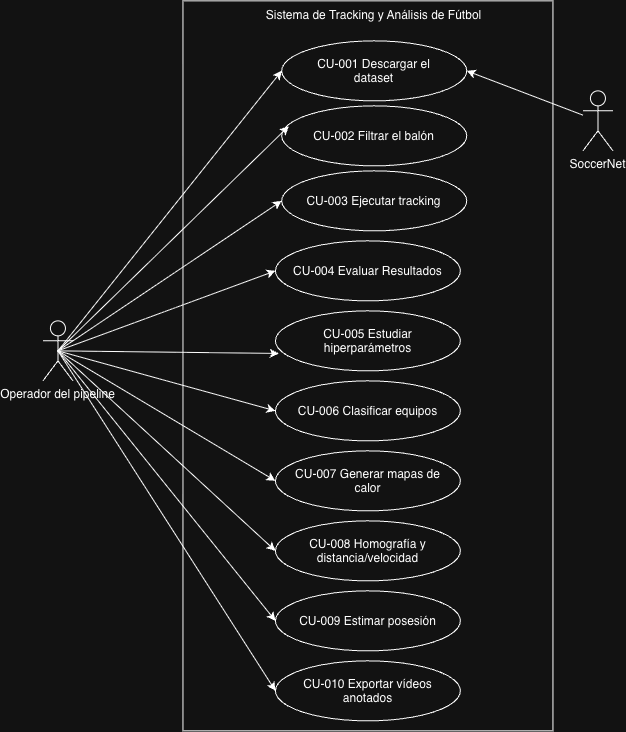
\includegraphics[width=0.9\textwidth]{figures/casosdeuso1.drawio.png}
\caption{Casos de uso del pipeline offline: el operador del pipeline y
SoccerNet como sistema externo.}
\label{fig:cu-pipeline}
\end{figure}

\begin{figure}[htp]
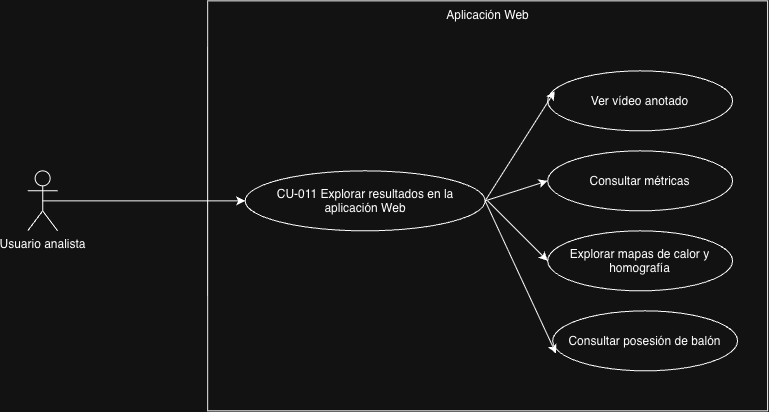
\includegraphics[width=0.9\textwidth]{figures/casosdeuso2.drawio.png}
\caption{Caso de uso de la aplicación web: el usuario analista
explora los resultados a través de cuatro comportamientos incluidos.}
\label{fig:cu-web}
\end{figure}

\begin{table}[htp]
\centering
\caption{CU-001: Descargar el dataset.}
\label{tab:cu-001}
\renewcommand{\arraystretch}{1.2}
\begin{tabular}{|p{3.1cm}|p{9.2cm}|}
\hline
\rowcolor{gray!25}
\multicolumn{2}{|l|}{\textbf{CU-001 -- Descargar el dataset}} \\
\hline
Actor & Operador del pipeline \\
\hline
Descripción & El operador ejecuta la descarga de las secuencias de
  SoccerNet-Tracking mediante la API oficial. \\
\hline
Precondiciones & Acceso a la API de SoccerNet. \\
\hline
Flujo principal & 1) El operador ejecuta
  \texttt{soccernet\_download.py}. 2) El sistema descarga las secuencias de
  train, test y \emph{challenge}. 3) Las almacena en la estructura de
  carpetas esperada por el resto del pipeline. \\
\hline
Postcondiciones & Dataset disponible localmente para el resto de casos de
  uso. \\
\hline
\end{tabular}
\end{table}

\begin{table}[htp]
\centering
\caption{CU-002: Filtrar el balón de las detecciones.}
\label{tab:cu-002}
\renewcommand{\arraystretch}{1.2}
\begin{tabular}{|p{3.1cm}|p{9.2cm}|}
\hline
\rowcolor{gray!25}
\multicolumn{2}{|l|}{\textbf{CU-002 -- Filtrar el balón de las detecciones}} \\
\hline
Actor & Operador del pipeline \\
\hline
Descripción & El sistema separa las detecciones de balón del resto antes de
  pasarlas al tracker. \\
\hline
Precondiciones & \texttt{det.txt} de la secuencia disponible. \\
\hline
Flujo principal & 1) El sistema lee cada detección del frame. 2) Calcula su
  área y su ratio ancho y alto. 3) La clasifica como balón o jugador según
  los umbrales del filtro geométrico. \\
\hline
Postcondiciones & Detecciones de jugadores separadas de las de balón, listas
  para el tracking. \\
\hline
\end{tabular}
\end{table}

\begin{table}[htp]
\centering
\caption{CU-003: Ejecutar tracking (ByteTrack / OC-SORT).}
\label{tab:cu-003}
\renewcommand{\arraystretch}{1.2}
\begin{tabular}{|p{3.1cm}|p{9.2cm}|}
\hline
\rowcolor{gray!25}
\multicolumn{2}{|l|}{\textbf{CU-003 -- Ejecutar tracking}} \\
\hline
Actor & Operador del pipeline \\
\hline
Descripción & El operador ejecuta uno o ambos algoritmos de tracking sobre
  una o todas las secuencias de un split. \\
\hline
Precondiciones & Detecciones de jugadores filtradas disponibles. \\
\hline
Flujo principal & 1) El operador lanza \texttt{run\_all\_train.py} o
  \texttt{run\_all\_test.py}. 2) El sistema inicializa el tracker
  elegido. 3) Actualiza el tracker frame a frame con las detecciones. 4)
  Persiste los resultados en formato MOT (IRQ-004). \\
\hline
Postcondiciones & Resultados de tracking disponibles para su evaluación. \\
\hline
\end{tabular}
\end{table}

\begin{table}[htp]
\centering
\caption{CU-004: Evaluar resultados de tracking.}
\label{tab:cu-004}
\renewcommand{\arraystretch}{1.2}
\begin{tabular}{|p{3.1cm}|p{9.2cm}|}
\hline
\rowcolor{gray!25}
\multicolumn{2}{|l|}{\textbf{CU-004 -- Evaluar resultados de tracking}} \\
\hline
Actor & Operador del pipeline \\
\hline
Descripción & El operador evalúa los resultados de tracking con
  \texttt{TrackEval}. \\
\hline
Precondiciones & Resultados de tracking y \emph{ground truth}
  disponibles. \\
\hline
Flujo principal & 1) El sistema genera el \emph{seqmap} del split. 2)
  Ejecuta \texttt{TrackEval} sobre los resultados de cada algoritmo. 3)
  Persiste las métricas por secuencia y combinadas. \\
\hline
Postcondiciones & Métricas de evaluación disponibles para la comparativa
  (capítulo~\ref{cap:pruebas}). \\
\hline
\end{tabular}
\end{table}

\begin{table}[htp]
\centering
\caption{CU-005: Realizar estudio de hiperparámetros.}
\label{tab:cu-005}
\renewcommand{\arraystretch}{1.2}
\begin{tabular}{|p{3.1cm}|p{9.2cm}|}
\hline
\rowcolor{gray!25}
\multicolumn{2}{|l|}{\textbf{CU-005 -- Realizar estudio de hiperparámetros}} \\
\hline
Actor & Operador del pipeline \\
\hline
Descripción & El operador ejecuta el barrido de hiperparámetros de un
  algoritmo y obtiene su configuración óptima. \\
\hline
Precondiciones & Detecciones de test filtradas y evaluación
  disponibles. \\
\hline
Flujo principal & 1) El sistema recorre cada valor del rango de un
  hiperparámetro. 2) Ejecuta el tracking y la evaluación con ese
  valor. 3) Registra la métrica resultante. 4) Selecciona el valor con
  mejor HOTA y lo confirma con una ejecución independiente (RF-008). \\
\hline
Postcondiciones & Configuración óptima determinada y validada para el
  algoritmo. \\
\hline
\end{tabular}
\end{table}

\begin{table}[htp]
\centering
\caption{CU-006: Clasificar jugadores por equipo.}
\label{tab:cu-006}
\renewcommand{\arraystretch}{1.2}
\begin{tabular}{|p{3.1cm}|p{9.2cm}|}
\hline
\rowcolor{gray!25}
\multicolumn{2}{|l|}{\textbf{CU-006 -- Clasificar jugadores por equipo}} \\
\hline
Actor & Operador del pipeline \\
\hline
Descripción & El operador ejecuta la clasificación de equipos por color de
  camiseta sobre una secuencia. \\
\hline
Precondiciones & Resultados de tracking con la configuración óptima
 disponibles. \\
\hline
Flujo principal & 1) El sistema recorta la zona de camiseta de cada
  detección de jugador. 2) Extrae su color dominante con K-means ($k=1$).
  3) Agrupa todos los colores en dos equipos con K-means ($k=2$). 4)
  Determina el equipo mayoritario de cada \texttt{track\_id}. \\
\hline
Postcondiciones & Asignación de equipo por jugador persistida. \\
\hline
\end{tabular}
\end{table}

\begin{table}[htp]
\centering
\caption{CU-007: Generar mapas de calor.}
\label{tab:cu-007}
\renewcommand{\arraystretch}{1.2}
\begin{tabular}{|p{3.1cm}|p{9.2cm}|}
\hline
\rowcolor{gray!25}
\multicolumn{2}{|l|}{\textbf{CU-007 -- Generar mapas de calor}} \\
\hline
Actor & Operador del pipeline \\
\hline
Descripción & El operador genera los mapas de calor de ocupación del
  campo, globales y por equipo. \\
\hline
Precondiciones & Resultados de tracking y, para el mapa por
  equipo, clasificación de equipos disponibles. \\
\hline
Flujo principal & 1) El sistema proyecta las posiciones de los jugadores
  sobre el campo dibujado a escala. 2) Calcula la densidad de posiciones
  mediante estimación KDE. 3) Genera y persiste la figura. \\
\hline
Postcondiciones & Mapas de calor disponibles. \\
\hline
\end{tabular}
\end{table}

\begin{table}[htp]
\centering
\caption{CU-008: Calcular homografía y estimar distancia/velocidad.}
\label{tab:cu-008}
\renewcommand{\arraystretch}{1.2}
\begin{tabular}{|p{3.1cm}|p{9.2cm}|}
\hline
\rowcolor{gray!25}
\multicolumn{2}{|l|}{\textbf{CU-008 -- Calcular homografía y estimar distancia/velocidad}} \\
\hline
Actor & Operador del pipeline \\
\hline
Descripción & El operador calcula una homografía real sobre un tramo
  verificado y estima distancia y velocidad de los jugadores. \\
\hline
Precondiciones & Tramo de cámara estable identificado manualmente
; resultados de tracking disponibles. \\
\hline
Flujo principal & 1) El operador identifica 4 puntos de referencia en un
  frame representativo. 2) El sistema calcula la matriz de homografía y
  valida su error de reproyección. 3) Proyecta las posiciones de cada
  jugador a metros reales. 4) Calcula distancia total y velocidad media y
  de pico. \\
\hline
Postcondiciones & Distancia y velocidad por jugador persistidas. \\
\hline
\end{tabular}
\end{table}

\begin{table}[htp]
\centering
\caption{CU-009: Estimar posesión de balón.}
\label{tab:cu-009}
\renewcommand{\arraystretch}{1.2}
\begin{tabular}{|p{3.1cm}|p{9.2cm}|}
\hline
\rowcolor{gray!25}
\multicolumn{2}{|l|}{\textbf{CU-009 -- Estimar posesión de balón}} \\
\hline
Actor & Operador del pipeline \\
\hline
Descripción & El operador calcula el porcentaje de posesión de balón por
  equipo, por proximidad espacial. \\
\hline
Precondiciones & Clasificación de equipos y detecciones de balón
 disponibles. \\
\hline
Flujo principal & 1) El sistema calcula, para cada frame con balón
  detectado, el jugador más cercano. 2) Comprueba que la distancia no
  supera el umbral. 3) Asigna la posesión de ese frame al equipo
  de ese jugador. 4) Agrega el resultado en porcentaje por equipo. \\
\hline
Postcondiciones & Porcentaje de posesión por equipo persistido. \\
\hline
\end{tabular}
\end{table}

\begin{table}[htp]
\centering
\caption{CU-010: Exportar vídeos anotados.}
\label{tab:cu-010}
\renewcommand{\arraystretch}{1.2}
\begin{tabular}{|p{3.1cm}|p{9.2cm}|}
\hline
\rowcolor{gray!25}
\multicolumn{2}{|l|}{\textbf{CU-010 -- Exportar vídeos anotados}} \\
\hline
Actor & Operador del pipeline \\
\hline
Descripción & El operador genera un vídeo con las cajas e identificadores
  de tracking superpuestos, para su uso en la memoria y en la demo. \\
\hline
Precondiciones & Resultados de tracking disponibles. \\
\hline
Flujo principal & 1) El operador selecciona secuencia y algoritmo. 2) El
  sistema dibuja las cajas e identificadores sobre cada frame. 3) Codifica
  el vídeo resultante en formato \texttt{.mp4}. \\
\hline
Postcondiciones & Vídeo anotado disponible en \texttt{videos/}. \\
\hline
\end{tabular}
\end{table}

\begin{table}[htp]
\centering
\caption{CU-011: Explorar resultados en la aplicación web.}
\label{tab:cu-011}
\renewcommand{\arraystretch}{1.2}
\begin{tabular}{|p{3.1cm}|p{9.2cm}|}
\hline
\rowcolor{gray!25}
\multicolumn{2}{|l|}{\textbf{CU-011 -- Explorar resultados en la aplicación web}} \\
\hline
Actor & Usuario analista \\
\hline
Descripción & El usuario explora los resultados del proyecto a través de
  dos vistas: una comparativa global de métricas entre algoritmos, y un
  explorador por secuencia y algoritmo con el vídeo anotado y los
  metadatos deportivos generados, sin recálculo en el navegador. Incluye:
  ver vídeo anotado, consultar métricas comparativas, explorar mapas de
  calor y homografía, y consultar posesión de balón. \\
\hline
Precondiciones & Datos de visualización exportados disponibles. \\
\hline
Flujo principal & 1) El usuario abre la aplicación web, que muestra por
  defecto la comparativa global de métricas entre algoritmos. 2) El
  usuario cambia a la pestaña de exploración por secuencias y selecciona
  secuencia y algoritmo. 3) La interfaz muestra el vídeo anotado y los
  paneles de equipos y posesión. 4) El usuario consulta, opcionalmente,
  los mapas de calor y la homografía de esa secuencia. \\
\hline
Postcondiciones & El usuario obtiene una interpretación visual de los
  resultados del proyecto, agregados o por secuencia concreta. \\
\hline
\end{tabular}
\end{table}

\section{Matriz de trazabilidad}
\label{sec:analisis-trazabilidad}

La matriz de trazabilidad relaciona los requisitos de este capítulo con los
objetivos específicos OE-01 a OE-11 definidos en la
sección~\ref{sec:intro-objetivos} del capítulo~\ref{cap:introduccion}.
Sirve para comprobar que cada objetivo queda cubierto por al menos un
requisito y que ningún requisito queda desligado de los fines del proyecto.
La trazabilidad se reparte en tres tablas, correspondientes a los
requisitos de información (Tabla~\ref{tab:traza-irq}), los requisitos
funcionales (Tabla~\ref{tab:traza-rf}) y los requisitos no funcionales
junto con las reglas de negocio (Tabla~\ref{tab:traza-rnf-rn}).

\begin{table}[htp]
\centering
\footnotesize
\caption{Trazabilidad de los requisitos de información.}
\label{tab:traza-irq}
\renewcommand{\arraystretch}{1.15}
\begin{tabular}{|p{1.3cm}|*{11}{>{\centering\arraybackslash}p{0.75cm}|}}
\hline
\rowcolor{gray!25}
\textbf{Req.} & \textbf{OE-01} & \textbf{OE-02} & \textbf{OE-03} & \textbf{OE-04} & \textbf{OE-05} & \textbf{OE-06} & \textbf{OE-07} & \textbf{OE-08} & \textbf{OE-09} & \textbf{OE-10} & \textbf{OE-11} \\
\hline
IRQ-001 & X & & & & & & & & & & \\
\hline
IRQ-002 & X & & & X & & & & & & & \\
\hline
IRQ-003 & X & & & & & & & & & & \\
\hline
IRQ-004 & & X & X & X & X & & & & & & \\
\hline
IRQ-005 & & & & X & X & & & & & & \\
\hline
IRQ-006 & & & & & X & & & & & & \\
\hline
IRQ-007 & & & & & & X & X & & X & & \\
\hline
IRQ-008 & & & & & & & X & X & X & & \\
\hline
IRQ-009 & & & & & & & & & & & X \\
\hline
\end{tabular}
\end{table}

\begin{table}[htp]
\centering
\footnotesize
\caption{Trazabilidad de los requisitos funcionales.}
\label{tab:traza-rf}
\renewcommand{\arraystretch}{1.15}
\begin{tabular}{|p{1.3cm}|*{11}{>{\centering\arraybackslash}p{0.75cm}|}}
\hline
\rowcolor{gray!25}
\textbf{Req.} & \textbf{OE-01} & \textbf{OE-02} & \textbf{OE-03} & \textbf{OE-04} & \textbf{OE-05} & \textbf{OE-06} & \textbf{OE-07} & \textbf{OE-08} & \textbf{OE-09} & \textbf{OE-10} & \textbf{OE-11} \\
\hline
RF-001 & X & & & & & & & & & & \\
\hline
RF-002 & & X & & & & & & & & & \\
\hline
RF-003 & & X & & & & & & & & & \\
\hline
RF-004 & & X & & & & & & & & & \\
\hline
RF-005 & & & X & & & & & & & & \\
\hline
RF-006 & & & & X & & & & & & & \\
\hline
RF-007 & & & & & X & & & & & & \\
\hline
RF-008 & & & & & X & & & & & & \\
\hline
RF-009 & & & & & X & & & & & & \\
\hline
RF-010 & & & & & & X & & & & & \\
\hline
RF-011 & & & & & & X & & & & & \\
\hline
RF-012 & & & & & & & X & & & & \\
\hline
RF-013 & & & & & & & & X & & & \\
\hline
RF-014 & & & & & & & & X & & & \\
\hline
RF-015 & & & & & & & & & X & & \\
\hline
RF-016 & & & & & & & & & & X & \\
\hline
RF-017 & & & & & & & & & & & X \\
\hline
\end{tabular}
\end{table}

\clearpage

\begin{table}[htp]
\centering
\footnotesize
\caption{Trazabilidad de requisitos no funcionales y reglas de negocio.}
\label{tab:traza-rnf-rn}
\renewcommand{\arraystretch}{1.15}
\begin{tabular}{|p{1.3cm}|*{11}{>{\centering\arraybackslash}p{0.75cm}|}}
\hline
\rowcolor{gray!25}
\textbf{Req.} & \textbf{OE-01} & \textbf{OE-02} & \textbf{OE-03} & \textbf{OE-04} & \textbf{OE-05} & \textbf{OE-06} & \textbf{OE-07} & \textbf{OE-08} & \textbf{OE-09} & \textbf{OE-10} & \textbf{OE-11} \\
\hline
RNF-001 & & & & & & & & & & X & \\
\hline
RNF-002 & & & X & & & & & & & & \\
\hline
RNF-003 & & & & & & & & & & X & \\
\hline
RNF-004 & & X & & & & & & & & & \\
\hline
RNF-005 & & & & & & & & & & X & \\
\hline
RNF-006 & & & & & & & & & & X & \\
\hline
RNF-007 & & & & & & & & & & & X \\
\hline
RNF-008 & & & & & & & & & & & X \\
\hline
RNF-009 & & & & & & & & & & & X \\
\hline
RN-001 & & X & & & & & & & & & \\
\hline
RN-002 & & & & X & & & & & & & \\
\hline
RN-003 & & & & & X & & & & & & \\
\hline
RN-004 & & & & & & X & & & & & \\
\hline
RN-005 & & & & & & & & X & & & \\
\hline
RN-006 & & & & & & & & & X & & \\
\hline
\end{tabular}
\end{table}

La lectura de las tres tablas muestra que los once objetivos específicos
reciben al menos una traza y que ningún requisito queda aislado. El
objetivo OE-10 (documentar las limitaciones técnicas)
recibe trazas exclusivamente de requisitos no funcionales, coherente con su
naturaleza transversal: no se satisface con una funcionalidad concreta,
sino con un criterio de calidad aplicado a todas las demás
(sección~\ref{sec:gestion-calidad}).
